%%%%%%%%%%%%%%%%%%%%%%%%%%%%%%%%%%%%%%%%%%%%%%%%%%%%%%%%%%%%%%%%%%%%%%%%%%%%%%%%%%%%%%%%%%%%%%%%%%%%%%%%%%%%%
% Inspired by last year's TACAS paper
%
%
% DEADLINE 
% Submission deadline for TACAS, FoSSaCS, FASE: October 10, 2024, 23:59 AoE
% TACAS mandatory artifact submission deadline: October 24, 2024
% Rebuttal (ESOP, FoSSaCS, partially TACAS): December 3–5, 2024
% Paper notification and TACAS mandatory artifact notification: December 20, 2024
%
% REQUIREMENTS:
% Info: https://etaps.org/2025/conferences/tacas/
% Formatting formatting guidelines must follow Springer’s LNCS (use the llncs.cls class)
% The review process of TACAS 2025 is single-blind.
% The length of regular research papers, case study papers, and regular tool papers is limited to 16 pp 
% excluding the bibliography and appendices.
% Additional material can be placed in a clearly marked appendix, at the end of the paper. 
% The reviewers are not obliged to read such appendices. 
% If the paper is accepted, a full version including the appendix should be made publicly available via arXiv or a similar platform.
%%%%%%%%%%%%%%%%%%%%%%%%%%%%%%%%%%%%%%%%%%%%%%%%%%%%%%%%%%%%%%%%%%%%%%%%%%%%%%%%%%%%%%%%%%%%%%%%%%%%%%%%%%%%%
\documentclass[runningheads]{llncs}

%%%%%%%%%%%%%%%%%%%%%%%%
% Imports
%%%%%%%%%%%%%%%%%%%%%%%%
% \usepackage{minted} % Package for syntax highlighting (https://ctan.org/pkg/minted)
\usepackage[T1]{fontenc} % Standard package for selecting font encodings (https://ctan.org/pkg/fontenc)
\usepackage{color}
\usepackage{hyperref} % Extensive support for hypertext in LATEX (https://ctan.org/pkg/hyperref)
\usepackage{graphicx} % Enhanced support for graphics (https://ctan.org/pkg/graphicx). Should include EPS figures.
\usepackage{cite}
\usepackage{subfig}
\usepackage{geometry} % Change page size at any point
\usepackage[edges]{forest} % Drat tree like data structures (https://ctan.org/pkg/forest)
\usepackage{pgffor} % Loops in LaTeX (https://ctan.org/pkg/pgffor)
\usepackage{csvsimple} % Simple CSV file processing (https://ctan.org/pkg/csvsimple)
\usepackage{underscore} % Control the behaviour of "_" in text (https://ctan.org/pkg/underscore)
\usepackage{listings} % Typeset source code listings using LATEX (https://ctan.org/pkg/listings)
\usepackage[title]{appendix}
\usepackage{adjustbox}
\usepackage{tikz}
\usepackage{xspace}
\usepackage{wrapfig}
\usepackage{amsmath}

%%%%%%%%%%%%%%%%%%%%%%%%
% Settings
%%%%%%%%%%%%%%%%%%%%%%%%
% \addto\extrasenglish{%
%     \providecommand*{\lstlistingautorefname}{List.}
%     % \renewcommand*{\listingscaption}{Code}
%     \renewcommand*{\equationautorefname}{Eq.}
%     \renewcommand*{\figureautorefname}{Fig.}
%     \renewcommand*{\chapterautorefname}{Chap.}
%     \renewcommand*{\sectionautorefname}{Sec.}
%     \renewcommand*{\subsectionautorefname}{Sub-sez.}
% }
\renewcommand\UrlFont{\color{blue}\rmfamily} % Change URL font
\urlstyle{rm} % Change URL style

%%%%%%%%%%%%%%%%%%%%%%%%
% References
%%%%%%%%%%%%%%%%%%%%%%%%
% \addbibresource{resources.bib} %Import the bibliography file

%%%%%%%%%%%%%%%%%%%%%%%%
% Glossary
%%%%%%%%%%%%%%%%%%%%%%%%
% \makeglossaries
% \loadglsentries{glossary}

%%%%%%%%%%%%%%%%%%%%%%%%
% Minted
%%%%%%%%%%%%%%%%%%%%%%%%
% \setminted[solidity]{tabsize=2,breaklines,fontsize=\footnotesize}
% \setminted[typescript]{tabsize=2,breaklines,fontsize=\footnotesize}


%%%%%%%%%%%%%%%%%%%%%%%%
% Geometry
%%%%%%%%%%%%%%%%%%%%%%%%
\newcommand{\framedtext}[1]{%
\par%
\noindent\fbox{%
    \parbox{\dimexpr\linewidth-2\fboxsep-2\fboxrule}{#1}%
}%
}

%%%%%%%%%%%%%%%%%%%%%%%%
% Listings
%%%%%%%%%%%%%%%%%%%%%%%%
\definecolor{keywords}{HTML}{C586C0}
\definecolor{type}{HTML}{0000FF}
\definecolor{operator}{HTML}{569CD6}
\definecolor{comments}{HTML}{6a9955}
\definecolor{variable}{HTML}{9e9b00}
\definecolor{number}{HTML}{098658}
\definecolor{function}{HTML}{795E26}

\lstset{language=C++,
    basicstyle=\ttfamily\small,
    keywordstyle=\color{keywords}\ttfamily,
    stringstyle=\color{orange}\ttfamily,
    commentstyle=\color{comments}\ttfamily,
    morecomment=[l][\color{comments}]{\#}
}
\lstdefinelanguage{SMT2}{
    alsoletter=-, % Include dashes as letters
    sensitive=true,
    morekeywords={set-logic, declare-fun, assert, check-sat, get-model},
    morekeywords=[2]{Int, Bool, Real},
    morekeywords=[3]{and, or, not, imply, ite},
    morekeywords=[4]{a, b, c, d, e, f, g, h, i, j, k, l, m, n, o, p, q, r, s, t, u, v, w, x, y, z},
    morecomment=[l]{;},
    morestring=[b]",
}
\lstset{
    language=SMT2,
    basicstyle=\ttfamily\small,
    keywordstyle=\color{keywords},
    keywordstyle={[2]\color{type}},
    keywordstyle={[3]\color{operator}},
    keywordstyle={[4]\color{variable}},
    commentstyle=\color{comments},
    stringstyle=\color{orange},
    showstringspaces=false,
    tabsize=2,
    breaklines=true,
}
\lstdefinelanguage{mps}{
    alsoletter=-, % Include dashes as letters
    sensitive=true,
    morekeywords={NAME, ROWS, COLUMNS, RHS, RANGES, BOUNDS, BINARIES, GENERALS, ENDATA},
    morekeywords=[2]{N, L, E, G, UP, LO, FX, FR, MI, PL},
    morecomment=[l]{*},
    morestring=[b]",
}
\lstset{
    language=mps,
    basicstyle=\ttfamily\small,
    keywordstyle=\color{keywords},
    keywordstyle={[2]\color{type}},
    commentstyle=\color{comments},
    stringstyle=\color{orange},
    showstringspaces=false,
    tabsize=2,
    breaklines=true,
}
\lstdefinelanguage{bazel}{
    alsoletter=-, % Include dashes as letters
    sensitive=true,
    morekeywords={load, workspace, http_archive, cc_binary, cc_library, cc_test, cc_toolchain, cc_toolchain_suite, filegroup, genrule, package_group, package, sh_binary, sh_library, sh_test},
    morekeywords=[2]{glob},
    morecomment=[l]{\#},
    morestring=[b]",
}
\lstset{
    language=bazel,
    basicstyle=\ttfamily\small,
    keywordstyle=\color{keywords},
    keywordstyle={[2]\color{function}},
    commentstyle=\color{comments},
    stringstyle=\color{orange},
    showstringspaces=false,
    tabsize=2,
    breaklines=true,
}
\lstdefinelanguage{yacc}{
    alsoletter={\#, \%, -, _, :}, % Include dashes as letters
    morekeywords={\#include, \#define, \#ifdef, \#endif},
    morekeywords=[2]{% Bison keywords
            \%union, \%token, \%type, \%nonassoc, \%left, \%prec, \%right, \%start,
            \%grammar, \%pure_parser, \%define, \%expect, \%expect-rr, \%file, \%glr-parser,
            \%parse-param, \%parse-param-rr, \%skeleton, \%debug, \%output,
            \%locations, \%skeleton
        },
    morekeywords=[3]{% Bison variables
            , stringVal,
        }
    keywordstyle=\color{keywords}\bfseries,
    morecomment=[l][\color{comments}]{//}, % single-line comments
    morecomment=[s][\color{comments}]{/*}{*/}, % multi-line comments
    morestring=[b]",
    morestring=[b]',
}
\lstset{
    language=yacc,
    basicstyle=\ttfamily\small,
    keywordstyle=\color{keywords},
    keywordstyle={[2]\color{type}},
    keywordstyle={[3]\color{variable}},
    commentstyle=\color{comments},
    stringstyle=\color{orange},
    showstringspaces=false,
    tabsize=2,
    breaklines=true,
}
\lstdefinelanguage{flex}{
    alsoletter={\#, \%, -, _, :}, % Include dashes as letters
    morekeywords={\#include, \#define, \#ifdef, \#endif},
    morekeywords=[2]{% Bison keywords
            typedef
        },
    morekeywords=[3]{% Bison variables
            , stringVal,
        }
    keywordstyle=\color{keywords}\bfseries,
    morecomment=[l][\color{comments}]{//}, % single-line comments
    morecomment=[s][\color{comments}]{/***}{*/}, % multi-line comments
    morestring=[b]",
    morestring=[b]',
}
\lstset{
    language=flex,
    basicstyle=\ttfamily\small,
    keywordstyle=\color{keywords},
    keywordstyle={[2]\color{type}},
    keywordstyle={[3]\color{variable}},
    commentstyle=\color{comments},
    stringstyle=\color{orange},
    showstringspaces=false,
    tabsize=2,
    breaklines=true,
}

%%%%%%%%%%%%%%%%%%%%%%%%
% Remove chapter header
%%%%%%%%%%%%%%%%%%%%%%%%
% \titleformat{\chapter}[display]{\normalfont\bfseries}{}{0pt}{\Huge}
% \newpagestyle{mystyle}
% {\sethead[\thepage][][\chaptertitle]{}{}{\thepage}}
% \pagestyle{mystyle}
% \AddToHook{env/appendices/begin}{%
%     \titleformat{\chapter}{\normalfont\LARGE\bfseries}{Appendix \thechapter}{10pt}{}%
% }

%%%%%%%%%%%%%%%%%%%%%%%%
% PlantUML
%%%%%%%%%%%%%%%%%%%%%%%%
\newcommand{\plantuml}[4][1]{
    \begin{figure}[h]
        \begin{adjustbox}{width=#1\textwidth,center}
            \input{#2}
        \end{adjustbox}
        \caption{#3}\label{dg:#4}
    \end{figure}
}

\newcommand{\wrapplantuml}[5][1]{
    \begin{wrapfigure}{#2}{#1\textwidth} %this figure will be at the right
        \centering
        \begin{adjustbox}{width=#1\textwidth,center}
            \input{#3}
        \end{adjustbox}
        \caption{#4}\label{dg:#5}
    \end{wrapfigure}
}

%%%%%%%%%%%%%%%%%%%%%%%%
% Common definitions
%%%%%%%%%%%%%%%%%%%%%%%%
\def\dlinear{\textit{dLinear}\xspace}
\def\pydlinear{\textit{pydLinear}\xspace}
\def\dlinearfive{\textit{dLinear5}\xspace}
\def\dlinearfour{\textit{dLinear4}\xspace}
\def\bazel{\textit{Bazel}\xspace}
\def\dreal{\textit{dReal4}\xspace}
\def\soplex{\textit{SoPlex}\xspace}


%%%%%%%%%%%%%%%%%%%%%%%%%%
% ---- Begin document ----
%%%%%%%%%%%%%%%%%%%%%%%%%%
\begin{document}

% ---- Metadata ----
\title{\dlinear: an SMT QF\_LRA Solver Supporting Floating Point Arithmetic and Delta-Completeness}
\titlerunning{\dlinear}

\author{Ernesto Casablanca\inst{1}
    %\orcidID{0009-0009-3741-1624}
    \and
    Martin Jonathan O'Connor Sidaway\inst{1}
    %\orcidID{0000-0001-6481-1169}
    \and
    Sadegh Soudjani\inst{2}
    %\orcidID{0000-0003-1922-6678}
    \and
    Paolo Zuliani\inst{3}
    %\orcidID{0000-0001-6481-1169}
}
\authorrunning{E. Casablanca et al.}

\institute{Newcastle University, Newcastle upon Tyne, United Kindgom\\
    \email{\{e.casablanca2,?martin?\}@newcastle.ac.uk} \and % TODO: add Martin's email and ensure orcidID
    Max Planck Institute for Software Systems, Kaiserslautern, Germany\\
    \email{sadegh@mpi-sws.org} \and
    La Sapienza University, Rome, Italy\\
    \email{zuliani@di.uniroma1.it}}

%%%%%%%%%%%%%%%%%%%%%
% ---- Sections ----
%%%%%%%%%%%%%%%%%%%%%

% ---- Title page ----
\maketitle

% ---- Abstract ----
\begin{abstract}
    This paper presents the first release of \dlinear, an open-source SMT solver for the QF\_LRA theory.
    Instead of relying on rational arithmetic to verify or disprove the linear constraints like most state-of-the-art SMT solvers, \dlinear uses cheaper floating-point arithmetic whenever possible while still guaranteeing an exact solution, ensuring the completeness of the solver.
    The tool also allows for $\delta$-complete reasoning, which relaxes the constraints by an arbitrary amount aiming to quicken the search for a model while ensuring that such a model, if it exists, will satisfy the original constraints within the given delta.
    This approach is extended to Neural Networks verification where the activation functions are piecewise linear.
    \dlinear is developed in C++ and can be used as a standalone tool or as a library.
    For ease of use, a Docker image and a Python interface, \textit{pydlinear}, are provided.
    We showcase the strengths of the tool on a set of benchmarks, comparing it to other well-known SMT solvers.

    \keywords{SMT \and Delta-complete \and Floating point arithmetic \and Neural Networks verification}
\end{abstract}

% ---- Introduction ----
\section{Introduction}

\gls{smt} has a notoriously vast variety of applications, ranging from formal software verification to planning and optimization just to name a few.
As expected, \gls{smt} solvers have received a lot of attention over the years, with some of the most well-known being cvc5~\cite{ref:cvc5}, Z3~\cite{ref:z3}, and Yices~\cite{ref:yices}.
Another field that is getting a lot of attention lately is Neural Networks.
Being an ever more pervasive presence in our everyday lives, formal verification of Neural Networks (NN) is quickly becoming a hot topic.
For this reason, multiple NN reasoners have been developed, including $\alpha$-$\beta$-CROWN~\cite{ref:a-crown,ref:b-crown,ref:crown,ref:lirpa}, Marabou~\cite{ref:marabou}, nnenum~\cite{ref:nnenum} and VeriNet~\cite{ref:verinet}.

The tool presented in this paper, \dlinear, is a \gls{qf-lra} \gls{smt} solver able produce both complete and $\delta$-complete outputs on standard \gls{smt} problems,
as well as tackling the verification of Neural Networks with piecewise linear activation functions.
While not as feature-rich as some of the other more mature \gls{smt} solvers yet, \dlinear is a first step in offering a different approach to \gls{smt} solving that can result in a significant speedup in some cases, especially when the theory solver constitutes the major performance bottleneck.

The paper is structured as follows: in \autoref{sec:preliminaries} we provide an overview of the theory behind \gls{smt}, with a focus on \gls{qf-lra} theory, and \gls{lp}.
In \autoref{sec:architecture} we give a technical description of the software architecture of the tool, with some details on the current support for neural network verification in \autoref{sec:nn-verification}.
The details of the algorithms used are analyzed more in-depth in \autoref{sec:lra-theory-solver}, which describes the approach we exploit to adapt the exact \gls{lp} solvers for \gls{smt} solving, and \autoref{sec:delta-completeness}, which defines $\delta$-completeness more formally.
Lastly, in \autoref{sec:benchmarks} we present the results of the experiments conducted to evaluate the performance of the tool.

\section{Preliminaries}
\label{sec:preliminaries}

\subsection{SAT and SMT}

A propositional formula is a construct that uses \textit{variables}, which are to be assigned a semantic value (i.e. \{\textbf{true}, \textbf{false}\}) and linked together by \textit{logical connectives} (i.e. $\lor$ (or), $\land$ (and) and $\neg$ (not)).
A literal is a variable (e.g. $x$) or its negation (e.g. $\neg x$).
Propositional formulae are usually expressed in the \gls{cnf}, which is to say as a conjunction of clauses, where a clause is a disjunction of literals \eqref{eq:cnf-notations}.
A generic propositional formula can be converted into an equisatisfiable \gls{cnf} formulation through the Tseitin encoding~\cite{ref:handbook-sat}.
\begin{equation}
    \label{eq:cnf-notations}
    \begin{gathered}
        \bigwedge_{i=1}^n \bigvee_{j=1}^{m_i} l_{ij} \\
        ( l_{00} \lor l_{01} \lor \dots \lor l_{0m_0}) \land (l_{10} \lor l_{11} \lor \dots \lor l_{1m_1}) \land \dots \land (l_{n0} \lor l_{n1} \lor \dots \lor l_{nm_n}) \\
        \{ \{ l_{00}, l_{01} , \dots , l_{0m_0} \} , \{ l_{10} , l_{11} , \dots , l_{1m_1} \}, \dots , \{ l_{n0} , l_{n1} , \dots , l_{nm_n} \} \}
    \end{gathered}
\end{equation}
\eqcaption{Three notations used to represent a CNF formula with $n$ clauses.}

A \gls{sat} solver is a procedure able to determine whether a given propositional formula is satisfiable, that is if it is possible to assign some boolean values to the variables that make the formula true.
Although the problem is generally NP complete~\cite{ref:np-sat}, over the years many efficient algorithms have been developed to tackle it, with the most popular being the \gls{cdlc} algorithm~\cite{ref:handbook-sat}, which started as an extension of the original \gls{dpll} algorithm~\cite{ref:dpll} with additional key techniques, such as learning clauses and from conflicts and exploiting their structure~\cite{ref:conflict-driven-clause-learning}, lazy data structures and low efficient branching heuristics~\cite{ref:watched-literals}.
\gls{cdlc} is employed in most recent state-of-the-art \gls{sat} solvers, such as the version of \textit{Minisat} in cvc5~\cite{ref:cvc5-smt-comp-2022} and \textit{Glucose}~\cite{ref:glucose}.

Satisfiability for propositional formulae can be extended to \gls{smt}.
Let $\Sigma$ be a signature containing predicate and function symbols, with an assigned arity $\ge 0$.
0-arity functions are called constants, while 0-arity predicates are propositions.
A term $t$ is defined as a constant or the application of a function symbol to a list of terms compatible with its arity.
A formula $\varphi$ can be a proposition, a predicate over a list of terms, or any logical connectives (e.g. $\land$, $\lor$, $\neg$, $\implies$) between formulae.
We also consider if-then-else ($ite$) terms, comprised of three elements: a formula and two terms.
\begin{equation}
    \label{eq:smt-notations}
    \begin{gathered}
        \begin{array}{lll}
            \Sigma^F         & \text{ functions } \in \Sigma                       \\
            \Sigma^P         & \text{ predicates } \in \Sigma                      \\
            \\
            c \in \Sigma^F   & \text{arity } 0                & \text{constant}    \\
            A \in \Sigma^P   & \text{arity } 0                & \text{proposition} \\
            f_n \in \Sigma^F & \text{arity } n > 0            & \text{function}    \\
            p_n \in \Sigma^P & \text{arity } n > 0            & \text{predicate}   \\
        \end{array}
        \\
        \begin{array}{lrll}
            t       & \coloneqq & c                                                                           & \text{term}    \\
                    & \mid      & f(t_1, \ldots, t_n)                                                                          \\
                    & \mid      & ite(\varphi, t_1, t_2)                                                                       \\
            \\
            \varphi & \coloneqq & A                                                                           & \text{formula} \\
                    & \mid      & p(t_1, \ldots, t_n)                                                                          \\
                    & \mid      & \neg\varphi    \mid \varphi_1 \land \varphi_2 \mid \varphi_1 \lor \varphi_2                  \\
                    & \mid      & \varphi_1 \implies \varphi_2 \mid \varphi_1 \iff \varphi_2                                   \\
        \end{array}
    \end{gathered}
\end{equation}
\eqcaption{Notations used to represent SMT terms and formulae.}
Formulae can be assigned a semantic meaning, \{\textbf{true}, \textbf{false}\}, by introducing a \textbf{model} $\mathcal{M}$, which is a pair $\{M, \mathcal{I}\}$ where $M$ is a non empty set and $\mathcal{I}$ is a mapping defined as follows:
\begin{gather*}
    \begin{array}{ll}
        \mathcal{I}(c)                      & = c^\mathcal{M} \in M                                                 \\
        \mathcal{I}(A)                      & = A^\mathcal{M} \in \{\textbf{true}, \textbf{false}\}                 \\
        \mathcal{I}(f_n)                    & = f^{\mathcal{M}} : M^n \rightarrow M                                 \\
        \mathcal{I}(p_n)                    & = p^{\mathcal{M}} : M^n \rightarrow \{\textbf{true}, \textbf{false}\} \\
        \mathcal{I}(f_n(t_1, \dots, t_n))   & = \mathcal{I}(f)(\mathcal{I}(t_1), \dots, \mathcal{I}(t_n))           \\
        \mathcal{I}(p_n(t_1, \dots, t_n))   & = \mathcal{I}(p)(\mathcal{I}(t_1), \dots, \mathcal{I}(t_n))           \\
        \mathcal{I}(ite(\varphi, t_1, t_2)) & = \begin{cases}
                                                    \mathcal{I}(t_1) & \text{if } \mathcal{I}(\varphi) = \textbf{true}  \\
                                                    \mathcal{I}(t_2) & \text{if } \mathcal{I}(\varphi) = \textbf{false}
                                                \end{cases}
    \end{array}
\end{gather*}
A model $\mathcal{M}$ \textbf{satisfies} a formula $\varphi$ if $\mathcal{I}(\varphi) = \textbf{true}$.

It is common to restrict the signature $\Sigma$ to a specific theory $\mathcal{T}$, such as the theory of linear real arithmetic (\textbf{QF\_LRA}), the theory of bit-vectors (\textbf{QF\_BV}), the theory of quantifier-free integer arithmetic (\textbf{QF\_NIA}), among many others~\footnote{SMT-LIB officially supported logics: \url{https://smt-lib.org/logics.shtml}}.
Then, the problem of \gls{smt} satisfiability is the problem of determining whether there exists a model that satisfies the formula $\varphi$ within the chosen theory.

The tool presented in this paper will focus on the \gls{qf-lra} theory.
The interpretation uses the domain $\bbbr$ of real numbers.
Only $+, -, \cdot,$ arithmetic operators are allowed, with the restriction that a variable can only be multiplied ($\cdot$) by a constant.
Therefore, each theory-literal in the formulae can be expressed in the form $a_1 \cdot x_1 + \ldots + a_n \cdot x_n \bowtie b$, where $x_i \in \bbbr \quad \forall i \in \{1, 2, \dots, n\}$ are variables, $a_i, b \in \bbbr \quad \forall i \in \{1, 2, \dots, n\}$ are constants and $\bowtie \in \{<, \le, =, \ne, \ge, >\}$.
With these restrictions in place, the \gls{qf-lra} theory is decidable.

\subsection{LP}
\label{sec:lp}

It is easy to see how the \gls{qf-lra} theory is very closely related to the \gls{lp} problem.
A linear program is a mathematical optimization problem where the objective function is to maximize, and the constraints the solution is subject to are linear.
Adopting a very common notation, consider a system of $m$ linear inequalities with unknown $x \in \bbbr^n$ and constant values $A \in \bbbr^{m \times n}$, $b \in \bbbr^m$ and $c \in \bbbr^n$.
Variables may be bounded by $l \in \bbbr^n$ and $u \in \bbbr^n$, such that $l_i \le x_i \le u_i \quad \forall i \in \{1, 2, \ldots, n\}$.
\gls{lp} problems are often presented in the \textit{standard form} \eqref{eq:lp-standard}, where the objective function is to be maximized, the constraints are all $\le$ inequalities and the variables are non-negative.
The conversion to the standard form is always possible and can be achieved in polynomial time.
\begin{equation}
    \label{eq:lp-standard}
    \begin{split}
        \text{Maximize }   \quad & \sum_{i=1}^{n} c_i x_i                      \\
        \text{subject to } \quad & \sum_{i=1}^{n} a_{ji}x_{i} < b_j            \\
        & x_i \ge 0,  \quad i \in \{1, 2, \ldots, n\}
    \end{split}
\end{equation}
\eqcaption{\gls{lp} problem in standard form.}

The most commonly used algorithm to solve \gls{lp} problems is the Simplex method~\cite{ref:simplex}.
Despite having a worst-case exponential time complexity, it is often very efficient in practice.

State-of-the-art \gls{smt} solvers such as Z3~\cite{ref:z3}, CVC5~\cite{ref:cvc5} and Yices~\cite{ref:yices} already fully support the \gls{qf-lra} theory
by employing a specialized Simplex-based~\cite{ref:simplex} solver with rational numerical representation to guarantee an exact solution and support strict inequalities.
Unfortunately, unlike floating point arithmetic, exact rational arithmetic does not offer constant time complexity when it comes to mathematical operations,
as the time required to complete the computations grows based on the size of the rational representation, which is only limited by the hardware's resources.
In the \gls{lp} community, a tradeoff between precision and speed of the tool usually favors the former, with many commercial tools utilizing floating point arithmetic~\cite{ref:gurobi} to achieve faster computations.
This is not considered a viable option in the \gls{smt} context: inexact procedures would not guarantee completeness, as rounding errors are introduced in the computation.

Some alternative methods have been developed over the years.
The \qsoptex solver \footnote{QSoptex: \url{https://www.math.uwaterloo.ca/~bico/qsopt/ex/index.html}} uses a technique called \textbf{incremental precision boosting}~\cite{ref:precision-boosting}.
Working with floating-point numbers with variable precision, the algorithm increments the number of bits used in their representation until the solution is found, then checks it using a rational number representation only to confirm its correctness.
A different approach is to utilize an \textbf{iterative refinement algorithm}~\cite{ref:iterative-refinement} such as the one implemented in \soplex~\cite{ref:soplex}.
This variation starts by solving the original problem with a fixed precision before considering a sequence of related \gls{lp} instances that only differ in the variables' bounds, the constraints' sides, and the objective function coefficients.
These subtasks translate in a shift/zoom of the original \gls{lp} instance, increasing the initial output's precision.
The process is iterated until the desired resolution is reached.
Some subroutines are in place to check for unsoundness and infeasibility in the presence of approximations derived from floating-point arithmetic.

% ---- Architecture ----
\section{Architecture}
\label{sec:architecture}

\dlinear implements the standard CDCL(T)-based~\cite{ref:dpll-t} \gls{smt} solver structure utilized in most other state-of-the-art solvers~\cite{ref:cvc5}.
CDCL(T)-based solvers follow the lazy approach to \gls{smt} solving, being comprised of two main components interacting with each other (see~\autoref{dg:dpll}): a boolean \textbf{\gls{sat} solver} and a specialized \textbf{Theory solver}.
All non-boolean formulae are first hidden behind a fresh corresponding boolean \textbf{theory-literal}.
The \gls{sat} solver aims to satisfy the problem by assigning a $true$ or $false$ value to each literal.
If no assignment is possible, we have determined the unsatisfiability of the input (I).
On the other hand, if a boolean model is returned, the theory solver checks the consistency of the theory-literals that have been assigned a value by building a \gls{lp} problem from the corresponding linear constraints and checking its feasibility.
If the problem is feasible, meaning the assignment is consistent with the theory, the model is returned, terminating the process (II).
Otherwise, the theory solver is responsible for generating an explanation, which takes the form of one or more learned clauses to add to the original input, forcing the \gls{sat} solver to backtrack and try a different assignment while ensuring the same model will not be selected again.
This process is repeated until one of the two exit conditions (I), (II) is met.
As long as the explanations produced by the theory solver do not loop and only contain a combination of the theory-literals enabled for that iteration, the solver will eventually terminate.

\plantuml[0.6]{diagrams/dpll}{CDCL(T)-based SMT solver}{dpll}

More formally, taking only the theory-literals into account, the assignment the \gls{sat} solver produces can be seen as the formula
\begin{equation} % Taken from Martin's thesis
    \label{eq:smt-formula}
    \varphi = t_1(x) \bowtie 0 \wedge \ldots \wedge t_m (x) \bowtie 0
\end{equation}
where
\begin{equation*}
    t_i(x) = a_{i1}x_1 + \ldots + a_{in}x_n - b_i, \quad 1 \le i \le m
\end{equation*}
with $A \in \bbbr^{m \times n}, b \in \bbbr^m$ and $\bowtie \in \{<, \le, =, \ne, \ge, >\}$.
To satisfy $\varphi$ means finding $x \in \bbbr^n $ such that that
\begin{equation*}
    t_1(x) \bowtie 0 \wedge \ldots \wedge t_m(x) \bowtie 0
\end{equation*}
which can be seen as an \gls{lp} problem where we are only interested in the feasibility of the constraints and bounds.

\dlinear includes some elementary preprocessing techniques that can guide the SAT solver and cheaply detect simple unsatisfiable linear constraints and produce a conflict clause without calling the \gls{lp} solver.
\dlinear supports MPS files, a standard format for \gls{lp} problems, by implicitly creating a single assertion the solver will try to satisfy.

\subsection{Simple Neural network verification}
\label{sec:nn-verification}

\begin{wrapfigure}[21]{R}{3cm}
    \captionsetup{font=small}
    \vspace{-2.3cm}
    \resizebox{1.04\linewidth}{!}{%
        % generated by Plantuml 1.2024.3       
\definecolor{plantucolor0000}{RGB}{245,245,245}
\definecolor{plantucolor0001}{RGB}{24,24,24}
\definecolor{plantucolor0002}{RGB}{0,0,0}
\definecolor{plantucolor0003}{RGB}{176,224,230}
\definecolor{plantucolor0004}{RGB}{255,192,203}
\definecolor{plantucolor0005}{RGB}{211,211,211}
\definecolor{plantucolor0006}{RGB}{210,180,140}
\definecolor{plantucolor0007}{RGB}{245,222,179}
\begin{tikzpicture}[yscale=-1
,every node/.style={scale=1.3}
,pstyle0/.style={color=plantucolor0001,fill=plantucolor0000,line width=0.5pt}
,pstyle1/.style={color=plantucolor0001,line width=1.5pt}
,pstyle2/.style={color=plantucolor0001,fill=plantucolor0003,line width=0.5pt}
,pstyle3/.style={color=plantucolor0001,fill=plantucolor0004,line width=0.5pt}
,pstyle7/.style={color=plantucolor0001,line width=1.0pt}
,pstyle8/.style={color=plantucolor0001,fill=plantucolor0001,line width=1.0pt}
]
\draw[pstyle0] (48.9179pt,28.0488pt) arc (180:270:17.0488pt) -- (65.9667pt,11pt) -- (96.2059pt,11pt) arc (270:360:17.0488pt) -- (113.2547pt,28.0488pt) -- (113.2547pt,28.0488pt) arc (0:90:17.0488pt) -- (96.2059pt,45.0977pt) -- (65.9667pt,45.0977pt) arc (90:180:17.0488pt) -- (48.9179pt,28.0488pt) -- cycle;
\node at (58.9179pt,21pt)[below right,color=black]{\textbf{Input}};
\draw[pstyle1] (39.7529pt,65.0977pt) -- (123.8392pt,65.0977pt);
\draw[pstyle2] (12.4196pt,102.082pt) arc (180:270:16.9844pt) -- (29.404pt,85.0977pt) -- (50.1019pt,85.0977pt) arc (270:360:16.9844pt) -- (67.0863pt,102.082pt) -- (67.0863pt,102.082pt) arc (0:90:16.9844pt) -- (50.1019pt,119.0664pt) -- (29.404pt,119.0664pt) arc (90:180:16.9844pt) -- (12.4196pt,102.082pt) -- cycle;
\node at (22.4196pt,95.0977pt)[below right,color=black]{Conv};
\draw[pstyle3] (11pt,156.0508pt) arc (180:270:16.9844pt) -- (27.9844pt,139.0664pt) -- (51.5215pt,139.0664pt) arc (270:360:16.9844pt) -- (68.5059pt,156.0508pt) -- (68.5059pt,156.0508pt) arc (0:90:16.9844pt) -- (51.5215pt,173.0352pt) -- (27.9844pt,173.0352pt) arc (90:180:16.9844pt) -- (11pt,156.0508pt) -- cycle;
\node at (21pt,149.0664pt)[below right,color=black]{ReLU};
\draw[pstyle2] (12.4196pt,210.0195pt) arc (180:270:16.9844pt) -- (29.404pt,193.0352pt) -- (50.1019pt,193.0352pt) arc (270:360:16.9844pt) -- (67.0863pt,210.0195pt) -- (67.0863pt,210.0195pt) arc (0:90:16.9844pt) -- (50.1019pt,227.0039pt) -- (29.404pt,227.0039pt) arc (90:180:16.9844pt) -- (12.4196pt,210.0195pt) -- cycle;
\node at (22.4196pt,203.0352pt)[below right,color=black]{Conv};
\draw[pstyle2] (96.5059pt,156.0508pt) arc (180:270:16.9844pt) -- (113.4903pt,139.0664pt) -- (134.1882pt,139.0664pt) arc (270:360:16.9844pt) -- (151.1725pt,156.0508pt) -- (151.1725pt,156.0508pt) arc (0:90:16.9844pt) -- (134.1882pt,173.0352pt) -- (113.4903pt,173.0352pt) arc (90:180:16.9844pt) -- (96.5059pt,156.0508pt) -- cycle;
\node at (106.5059pt,149.0664pt)[below right,color=black]{Conv};
\draw[pstyle1] (39.7529pt,247.0039pt) -- (123.8392pt,247.0039pt);
\draw[color=plantucolor0001,fill=plantucolor0005,line width=0.5pt] (56.8063pt,283.9883pt) arc (180:270:16.9844pt) -- (73.7906pt,267.0039pt) -- (88.3819pt,267.0039pt) arc (270:360:16.9844pt) -- (105.3663pt,283.9883pt) -- (105.3663pt,283.9883pt) arc (0:90:16.9844pt) -- (88.3819pt,300.9727pt) -- (73.7906pt,300.9727pt) arc (90:180:16.9844pt) -- (56.8063pt,283.9883pt) -- cycle;
\node at (66.8063pt,277.0039pt)[below right,color=black]{Add};
\draw[pstyle3] (52.3333pt,337.957pt) arc (180:270:16.9844pt) -- (69.3177pt,320.9727pt) -- (92.8548pt,320.9727pt) arc (270:360:16.9844pt) -- (109.8392pt,337.957pt) -- (109.8392pt,337.957pt) arc (0:90:16.9844pt) -- (92.8548pt,354.9414pt) -- (69.3177pt,354.9414pt) arc (90:180:16.9844pt) -- (52.3333pt,337.957pt) -- cycle;
\node at (62.3333pt,330.9727pt)[below right,color=black]{ReLU};
\draw[color=plantucolor0001,fill=plantucolor0006,line width=0.5pt] (57.9819pt,391.9258pt) arc (180:270:16.9844pt) -- (74.9663pt,374.9414pt) -- (87.2062pt,374.9414pt) arc (270:360:16.9844pt) -- (104.1906pt,391.9258pt) -- (104.1906pt,391.9258pt) arc (0:90:16.9844pt) -- (87.2062pt,408.9102pt) -- (74.9663pt,408.9102pt) arc (90:180:16.9844pt) -- (57.9819pt,391.9258pt) -- cycle;
\node at (67.9819pt,384.9414pt)[below right,color=black]{Pad};
\draw[color=plantucolor0001,fill=plantucolor0007,line width=0.5pt] (44.8226pt,445.8945pt) arc (180:270:16.9844pt) -- (61.807pt,428.9102pt) -- (100.3655pt,428.9102pt) arc (270:360:16.9844pt) -- (117.3499pt,445.8945pt) -- (117.3499pt,445.8945pt) arc (0:90:16.9844pt) -- (100.3655pt,462.8789pt) -- (61.807pt,462.8789pt) arc (90:180:16.9844pt) -- (44.8226pt,445.8945pt) -- cycle;
\node at (54.8226pt,438.9102pt)[below right,color=black]{Flatten};
\draw[pstyle0] (43.3189pt,499.9277pt) arc (180:270:17.0488pt) -- (60.3678pt,482.8789pt) -- (101.8048pt,482.8789pt) arc (270:360:17.0488pt) -- (118.8536pt,499.9277pt) -- (118.8536pt,499.9277pt) arc (0:90:17.0488pt) -- (101.8048pt,516.9766pt) -- (60.3678pt,516.9766pt) arc (90:180:17.0488pt) -- (43.3189pt,499.9277pt) -- cycle;
\node at (53.3189pt,492.8789pt)[below right,color=black]{\textbf{Output}};
\draw[pstyle7] (39.7529pt,119.0664pt) -- (39.7529pt,139.0664pt);
\draw[pstyle8] (35.7529pt,129.0664pt) -- (39.7529pt,139.0664pt) -- (43.7529pt,129.0664pt) -- (39.7529pt,133.0664pt) -- cycle;
\draw[pstyle7] (39.7529pt,173.0352pt) -- (39.7529pt,193.0352pt);
\draw[pstyle8] (35.7529pt,183.0352pt) -- (39.7529pt,193.0352pt) -- (43.7529pt,183.0352pt) -- (39.7529pt,187.0352pt) -- cycle;
\draw[pstyle7] (39.7529pt,66.5977pt) -- (39.7529pt,85.0977pt);
\draw[pstyle8] (35.7529pt,75.0977pt) -- (39.7529pt,85.0977pt) -- (43.7529pt,75.0977pt) -- (39.7529pt,79.0977pt) -- cycle;
\draw[pstyle7] (123.8392pt,66.5977pt) -- (123.8392pt,139.0664pt);
\draw[pstyle8] (119.8392pt,129.0664pt) -- (123.8392pt,139.0664pt) -- (127.8392pt,129.0664pt) -- (123.8392pt,133.0664pt) -- cycle;
\draw[pstyle7] (39.7529pt,227.0039pt) -- (39.7529pt,247.0039pt);
\draw[pstyle8] (35.7529pt,237.0039pt) -- (39.7529pt,247.0039pt) -- (43.7529pt,237.0039pt) -- (39.7529pt,241.0039pt) -- cycle;
\draw[pstyle7] (123.8392pt,173.0352pt) -- (123.8392pt,247.0039pt);
\draw[pstyle8] (119.8392pt,237.0039pt) -- (123.8392pt,247.0039pt) -- (127.8392pt,237.0039pt) -- (123.8392pt,241.0039pt) -- cycle;
\draw[pstyle7] (81.0863pt,45.0977pt) -- (81.0863pt,65.0977pt);
\draw[pstyle8] (77.0863pt,55.0977pt) -- (81.0863pt,65.0977pt) -- (85.0863pt,55.0977pt) -- (81.0863pt,59.0977pt) -- cycle;
\draw[pstyle7] (81.0863pt,248.5039pt) -- (81.0863pt,267.0039pt);
\draw[pstyle8] (77.0863pt,257.0039pt) -- (81.0863pt,267.0039pt) -- (85.0863pt,257.0039pt) -- (81.0863pt,261.0039pt) -- cycle;
\draw[pstyle7] (81.0863pt,300.9727pt) -- (81.0863pt,320.9727pt);
\draw[pstyle8] (77.0863pt,310.9727pt) -- (81.0863pt,320.9727pt) -- (85.0863pt,310.9727pt) -- (81.0863pt,314.9727pt) -- cycle;
\draw[pstyle7] (81.0863pt,354.9414pt) -- (81.0863pt,374.9414pt);
\draw[pstyle8] (77.0863pt,364.9414pt) -- (81.0863pt,374.9414pt) -- (85.0863pt,364.9414pt) -- (81.0863pt,368.9414pt) -- cycle;
\draw[pstyle7] (81.0863pt,408.9102pt) -- (81.0863pt,428.9102pt);
\draw[pstyle8] (77.0863pt,418.9102pt) -- (81.0863pt,428.9102pt) -- (85.0863pt,418.9102pt) -- (81.0863pt,422.9102pt) -- cycle;
\draw[pstyle7] (81.0863pt,462.8789pt) -- (81.0863pt,482.8789pt);
\draw[pstyle8] (77.0863pt,472.8789pt) -- (81.0863pt,482.8789pt) -- (85.0863pt,472.8789pt) -- (81.0863pt,476.8789pt) -- cycle;
\end{tikzpicture}

    }
    \caption{ONNX graph.}
    \label{dg:onnx}
\end{wrapfigure}

\dlinear supports a naive algorithm to verify neural networks that utilize ReLU activation functions.
Given an \gls{onnx} file~\footnote{\url{https://onnx.ai/index.html}}, the acyclic graph describing the network with all its layers is parsed, from inputs to outputs~(\autoref{dg:onnx}).
Exploring the graph, most of the layers are converted into linear constraints that can be handled by the \dlinear's \gls{smt} solver functionalities.
Upon encountering a piecewise linear activation function, we declare a fresh variable $y'$ and introduce enough formula to assert its equality with each of the possible outputs of the activation function.
These new formulae are then added to the set of assertions in an "at most one" encoding.
From that point on, $y'$ replaces the corresponding linear constraint for all the dependent nodes of the graph.
For instance, the ReLU activation function can be represented as
\begin{equation*}
    y' = \begin{cases}
        x & \text{if } x \ge 0 \\
        0 & \text{otherwise}
    \end{cases}
\end{equation*}
Given the two new formulae $A \coloneqq (y' = x), B \coloneqq (y' = 0)$, the clauses $(A \lor B) \land (\neg A \lor \neg B)$ are added to the set of assertions.

Even limiting ourselves to the common ReLU activation layer, the number of subproblems grows exponentially, making the verification process computationally intractable even for medium-sized networks.
To mitigate this issue, we can try to exploit the structure of the problem.
The bound propagation mentioned in Section~\ref{sec:preprocessing} is adapted to iteratively tighten the bounds of the output of each activation layer.
In the best case, the newly found bounds can uniquely indicate the only branch a piecewise function can take, effectively removing the need to explore the other branches.
Furthermore, constraints coming from activation functions are encoded as a \gls{soi}, which becomes the objective function to minimize while the other linear expression creates the constraints the problem is subject to.
Note that some additional constraints may be needed to ensure the two formulations are equivalent.
In the case of ReLUs, we must also enforce that the output of the activation function is greater than or equal to the input, which can be achieved by adding the constraints $y' \ge x$.
If the solver finds a solution where the objective value is equal to $0$, then we obtain a valid model.
If the objective value is greater than $0$, we can guide the solver by suggesting the inversion of the activation function which has the highest cost, defined as its absolute value given the current solution vector.

% ---- Linear Real Arithmetic theory ----
\section{Linear Real Arithmetic theory solver}
\label{sec:lra-theory-solver}

\subsection*{Preprocessing}
\label{sec:preprocessing}

\dlinear implements some of the common preprocessing strategies when it comes to optimizing the performance solver for the \gls{qf-lra} theory.
The first step is to add some inexpensive implications between the bounds on the same variable, such as $x \ge 1 \implies x \ge 0 \implies x \ge -10$, potentially avoiding pointless assignments from the SAT solver.
Then, all simple equality bounds are propagated using the problem's constraints, in a process that can be visualized as a graph-like structure (\autoref{dg:preprocessor}).
If one or more conflicts are detected, the original atoms are traced back and used to generate the explanations.
If no conflict is detected, the bounds are propagated to the variables, potentially inducing stronger bounds.
The user can limit the preprocessing engine to only run once, on the fixed theory literals, instead of at every iteration, or they can disable it completely if its contribution is deemed to be negligible or even detrimental to the overall performance on the given instance.

\begin{figure}[h]
    \begin{tikzpicture}
        \begin{scope}[every node/.style={rectangle,thick,draw}]
            \node (1) at (0,4) {$x_1 = 1$};
            \node[shape=rectangle,draw=none] (a) at (3,3) {$x_1 + x_2 + x_4 = 7$};
            \node (2) at (0,2) {$x_2 = 2$};
            \node (3) at (0,0) {$x_3 = 3$};
            \node[shape=rectangle,draw=blue] (4) at (6,3) {$x_4 = 4$};
            \node[shape=rectangle,draw=blue] (5) at (6,1) {$x_5 = 5$};
            \node[draw=red] (6) at (12,2) {$x_6 = 6 \land x_6 = 7$};
        \end{scope}

        \begin{scope}[>={Stealth[black]},
            every node/.style={fill=white,rectangle},
            every edge/.style={draw=black,very thick}]
            \path [-] (1) edge (a);
            \path [-] (2) edge (a);
            \path [->] (a) edge (4);
            \path [->] (1) edge[bend left=20] node {$3x_1 -  x_4 = 1$} (4);
            \path [->] (3) edge[draw=red] node {$x_3 + 2x_5 = 13$} (5);
            \path [->] (2) edge[draw=red] node {$-3x_2 + x_6 = 0$} (6);
            \path [->] (5) edge[draw=red] node {$-7x_5 + x_6 = -28$} (6);
        \end{scope}
    \end{tikzpicture}
    \caption{Example of a preprocessor graph. The given bounds (the nodes on the left) propagate using the constraints, inducing additional bounds (the blue nodes) that can be used to guide the solver.
        If a conflict is detected (red node), the edges responsible (red edges) are traced back to the origin to formulate an explanation to add to the SAT solver.
        In this case, the explanation adds the clause $(\neg l_1 \lor \neg l_2 \lor \neg l_3 \lor \neg l_4 \lor \neg l_5)$ where $l_1 \coloneqq x_2 = 2, l_2 \coloneqq x_3 = 3, l_3 \coloneqq -3x_2 + x_6 = 0, l_4 \coloneqq x_3 + 2x_5 = 13, l_5 \coloneqq -7x_5 + x_6 = -28$.
        All new valid assignments will not have all three red edges.}
    \label{dg:preprocessor}
\end{figure}

\subsection{LP solver}

\dlinear uses \soplex as its default \gls{lp} solver.
It implements both the incremental precision boosting and the iterative refinement algorithms.
The user can choose between the two or try a hybrid approach.
\qsoptex can be used as an alternative solver, but it is limited to precision boosting and tends to produce less compact explanations, leading to more conflicts and slower convergence.

If a feasible solution is found, it means that the original formula is satisfiable, and the assignment is returned to the user.
Note that the solution's uniqueness is not guaranteed, so adding an artificial clause with the negation of the solution found will force the solver to find another assignment, if possible.
On the other hand, if the \gls{lp} problem is infeasible, we can use the Farkas proof $y \in \bbbr^m$, corresponding to the last feasible solution of the dual problem before its unboundedness or infeasibility was detected.
Given the initial $Ax \le b$ and $l \le x \le u$, we get an inequality $y^T A x \le y^T b$, which is infeasible over the local bounds, meaning that even setting $x_i$ to the bound that minimizes $y^T A$, the result will still be $y^T A x > y^T b$.
Collecting the constraints corresponding to the indexes where the Farkas proof is non-zero and the minimizing bounds makes it possible to determine a small infeasible subsystem of the original problem, albeit not necessarily an irreducible one, and use it to produce an explanation.

\subsection{Strict bounds}
\label{sec:strict-bounds}

To use out-of-the-box \gls{lp} solvers as theory solvers, some adjustments in the formulation of the input may be required.
Strict inequalities are common in \gls{smt} formulae, but they are usually not supported by \gls{lp} solvers.
They would make the feasible region no longer closed, possibly making the search for the optimal solution pointless.
Other state-of-the-art \gls{smt} solver employing rational arithmetic within the theory solver~\footnote{z3 documentation: \url{https://z3prover.github.io/papers/z3internals.html\#sec-rational-linear-arithmetic}}, use a symbolic variable representing an infinitesimal parameter $\delta$ which enforces the inequality~\cite{ref:lra-dpll-t}.
Since our goal is to verify feasibility, we can reformulate the problem into an equi-feasible one while eliminating the strict inequalities at the cost of losing the original objective function, which is not relevant in this context anyway.
We introduce a new variable called \textbf{strict variable}, $t$.
To simplify the notation, we only consider $<$ strict inequalities, but the same reasoning can be applied to $>$ since they can always be converted to $<$ by multiplying both sides by $-1$.
The same applies to $\ge$ and $=$, which can be converted to $\le$ by using the standard form of the problem, as discussed in Section~\ref{sec:lp}.
Note that we are excluding \nqcs for now, as they will be discussed next.
Let $K$ indicate the set of indexes of strict inequality constraints ($<$) and with $J$ the set of indexes for all other constraints ($\le$).
Note that $K$ and $J$ are disjoint sets.
Without loss of generality, assume that all the indices in $K$ are less than those in $J$ ($\max(J) < \min(K)$).
Using intuitive indexing over vector and matrix elements, start by replacing each strict inequality
\begin{align*}
    \sum_{i=1}^{n} a_{ki}x_{i} < b_k, \quad \forall k \in K
\end{align*}
with equivalent non-strict inequalities using the strict variable $t$:
\begin{align*}
    \sum_{i=1}^{n} a_{ki}x_{i} + t \le b_k, \quad \forall k \in K \\
    t > 0
\end{align*}
This change would only move the strict inequality problem to the bound on $t$.
However, it is possible to go a step further and relax the newly introduced bound by changing the objective function to maximize $t$.
The original problem we want to verify the feasibility of
\begin{equation}
    \label{eq:lp-original}
    \begin{split}
        \text{Maximize }   \quad & 0                                                          \\
        \text{subject to } \quad & \sum_{i=1}^{n} a_{ji}x_{i} \le b_j,  \quad \forall j \in J \\
        \quad                    & \sum_{i=1}^{n} a_{ki}x_{i} < b_k,   \quad \forall k \in K  \\
        & l_i \le x_i \le u_i,  \quad i \in \{1, 2, \ldots, n\}
    \end{split}
\end{equation}
can be relaxed to
\begin{equation}
    \label{eq:lp-relaxed}
    \begin{split}
        \text{Maximize }   \quad & t                                                             \\
        \text{subject to } \quad & \sum_{i=1}^{n} a_{ji}x_{i} \le b_j, \quad \forall j \in J     \\
        \quad                    & \sum_{i=1}^{n} a_{ki}x_{i} + t \le b_k, \quad \forall k \in K \\
        & l_i \le x_i \le u_i,  \quad i \in \{1, 2, \ldots, n\},        \\
        & t \ge 0
    \end{split}
\end{equation}

\begin{theorem}
    \label{thm:lp-relaxed}
    The original problem \eqref{eq:lp-original} is feasible if and only if the relaxed problem \eqref{eq:lp-relaxed} is feasible and there exists a solution that satisfies its optimal value is strictly greater than $0$.
\end{theorem}

\subsection{Not equal to constraints}

Not equal to ($\ne$) constraints (\nqcs for short) pose a more significant challenge.
Let $D$ be the set of indexes of the \nqcs.
Again, without loss of generality, assume that all the indices in $D$ are greater than those in $K$ ($\max(K) < \min(D)$).
The extended relaxed problem is defined as
\begin{equation}
    \label{eq:lp-extended}
    \begin{split}
        \text{Maximize }   \quad & t                                                             \\
        \text{subject to } \quad & \sum_{i=1}^{n} a_{ji}x_{i} \le b_j, \quad \forall j \in J     \\
        \quad                    & \sum_{i=1}^{n} a_{ki}x_{i} + t \le b_k, \quad \forall k \in K \\
        \quad                    & \sum_{i=1}^{n} a_{di}x_{i} + t \le b_d, \quad \forall d \in D \\
        & l_i \le x_i \le u_i,  \quad i \in \{1, 2, \ldots, n\}         \\
        & t \ge 0
    \end{split}
\end{equation}

Two strict inequalities are needed to check whether the constraint is satisfied.
Since checking both simultaneously with an OR disjunction is not supported by the \gls{lp} solver, the original problem must be split into two subproblems.
Hence, given $|D|$ \nqcs, $2^{|D|}$ sub-problems are produced~\eqref{eq:nq}.
\begin{equation}
    \label{eq:nq}
    \begin{gathered}
        \begin{cases}
            A_{1 \dots |J|} x \le b_{1 \dots |J| - 1}                 \\
            A_{|J| + 1\dots |J| + |K|} x < b_{|J| + 1\dots |J| + |K|} \\
            A_{|J| + |K| + 1} x \ne b_{|J| + |K| + 1}                 \\
            A_{|J| + |K| + 2} x \ne b_{|J| + |K| + 2}                 \\
        \end{cases}
        \\
        \text{will be split into}
        \\
        \begin{pmatrix}
            \begin{cases}
                A_{1 \dots |J|} x \le b_{1 \dots |J| - 1}                 \\
                A_{|J| + 1\dots |J| + |K|} x < b_{|J| + 1\dots |J| + |K|} \\
                A_{|J| + |K| + 1} x < b_{|J| + |K| + 1}                   \\
                A_{|J| + |K| + 2} x < b_{|J| + |K| + 2}
            \end{cases}
             &
            \begin{cases}
                A_{1 \dots |J|} x \le b_{1 \dots |J| - 1}                 \\
                A_{|J| + 1\dots |J| + |K|} x < b_{|J| + 1\dots |J| + |K|} \\
                A_{|J| + |K| + 1} x < b_{|J| + |K| + 1}                   \\
                A_{|J| + |K| + 2} x > b_{|J| + |K| + 2}
            \end{cases}
            \\
            \begin{cases}
                A_{1 \dots |J|} x \le b_{1 \dots |J| - 1}                 \\
                A_{|J| + 1\dots |J| + |K|} x < b_{|J| + 1\dots |J| + |K|} \\
                A_{|J| + |K| + 1} x > b_{|J| + |K| + 1}                   \\
                A_{|J| + |K| + 2} x < b_{|J| + |K| + 2}
            \end{cases}
             &
            \begin{cases}
                A_{1 \dots |J|} x \le b_{1 \dots |J| - 1}                 \\
                A_{|J| + 1\dots |J| + |K|} x < b_{|J| + 1\dots |J| + |K|} \\
                A_{|J| + |K| + 1} x > b_{|J| + |K| + 1}                   \\
                A_{|J| + |K| + 2} x > b_{|J| + |K| + 2}
            \end{cases}
        \end{pmatrix}
    \end{gathered}
\end{equation}
\eqcaption{Splitting an LP problem with 2 \nqcs into 4 subproblems. Note that the \nqcs appear in $4$ configurations: $\{<, <\}, \{<, >\}, \{>, <\}, \{>, >\}$.}

If any of the subproblems is feasible, then it is possible to conclude that the original problem is feasible.
On the other hand, in the worst case, all $2^{|D|}$ problems must be solved to prove infeasibility.
Some smarter heuristics can improve the average performance of the solver.
For instance, there is no need to continue solving subproblems if none of the \nqcs are involved in the infeasibility.
Furthermore, if only precisely one of them appears in the explanation, we can skip all other subproblems where it appears with the same sense, for they will surely be infeasible too.
Also, we often only need to explore part of the tree to determine infeasibility.
If we find a subset of the \nqc that makes the problem infeasible on its own, we can immediately terminate the exploration.
We can obtain this early termination by enumerating the number of times a unique configuration of such a subset is solved.
If that number is equal to $2^{|T|}$, where $T$ is the set of indexes of the \nqcs in the subset, we can return an infeasibility explanation obtained by merging all the explanations produced by the subproblems that were enumerated.
Lastly, it is possible to \textit{hot start} the solver by starting in a configuration close to the one that caused the last infeasibility.

\subsection{Theory solver algorithm}

Let $\text{LpSolve}$ be a routine that, given a generic \gls{lp} problem and the set of indexes corresponding to the senses of the constraints ($\le, <, \ne$), solves the extended relaxed problem \eqref{eq:lp-extended} and returns the set of indexes of infeasible constraints if there are any or an empty set otherwise.
$\odot$ represents an element-wise multiplication between two vectors or a vector and a scalar, with the scalar repeated to match the size of the vector.
We adapt the \gls{lp} solver to the \gls{smt} context using the Algorithm~\ref{alg:theory-solver}.
To simplify the presentation, only the essential heuristics are included in the pseudocode.
\begin{algorithm}
    \caption{SMT adapted LP solver}\label{alg:theory-solver}
    \begin{algorithmic}
        \Require $A \in \bbbr^{(|J| + |K| + |D|) \times n}, b \in \bbbr^{|J| + |K| + |D|}, l \in \bbbr^n, u \in \bbbr^n$ \\
        \qquad as defined in~\autoref{sec:lp} over the extended relaxed problem~\eqref{eq:lp-extended}
        \Require $J, K, D$ as defined in~\autoref{sec:strict-bounds} \\
        \qquad note that $\max(J) < \min(K) \le \max(K) < \min(D)$
        \Ensure Set of indexes of infeasible constraints $E$ or $\emptyset$
        \State $E \gets \text{LpSolve}(A, b, l, u, J, K, \emptyset)$ \Comment{Solve the LP problem without $\ne$ constraints}
        \If{$E \ne \emptyset$}
        \State \Return $E$
        \EndIf
        \For {$s \in \text{ all non empty subsets of } D$}
        \State $V_s \gets \emptyset$
        \State $E_s \gets \emptyset$
        \EndFor
        \State $c \gets 0$ \Comment{Initialize the binary counter}
        \While{$c \le 2^{|D|}$}
        \State Let $C \in \{-1, 1\}^{|D|}$ be the binary representation of $c$ with $0$ replaced by $-1$
        \State $C' \in \{-1, 1\}^{|J|+|K|+|D|} \gets \begin{bmatrix} 1^{|J|} & 1^{|K|} & C\end{bmatrix}$
        \State $A' \gets \begin{bmatrix}A_1 \odot C'_1 \\ \vdots \\ A_{|J|+|K|+|D|} \odot C'_{|J|+|K|+|D|}\end{bmatrix}$
        \State $E \gets \text{LpSolve}(A', b \odot C', l, u, J, K, D)$
        \If{$E = \emptyset$} \Comment{At least one subproblem is feasible}
        \State \Return $\emptyset$
        \EndIf
        \State $T \gets E \cap D$
        \If{$T = \emptyset$} \Comment{No \nqcs are involved in the infeasibility, the problem is infeasible}
        \State \Return $E$
        \EndIf
        \State $l \gets \{ C'_{|J| + |K| + t} \mid \forall t \in T\}$ % I want to construct a vector where each element is defined by the corresponding element in C' if the index is in T
        \If{$l \in V_T$} \Comment{Avoid adding redundant explanations for the same infeasibility}
        \State \textbf{Continue}
        \EndIf
        \State $V_T \gets V_T \cup \{l\}$
        \State $E_T \gets E_T \cup E$
        \If{$|V_T| = 2^{|T|}$} \Comment{Having explored it fully, a subset of the $\ne$ constraints is infeasible}
        \State \Return $E_T$
        \EndIf
        \State $c \gets c + 1$
        \EndWhile
        \State \Return $E$
    \end{algorithmic}
\end{algorithm}

% ---- Delta-completeness ----
\section{$\delta$-completeness}
\label{sec:delta-completeness}

\dlinear offers the option to use $\delta$-completeness.
In this mode, the user can specify a precision parameter $\delta > 0$, relaxing the constraints to allow for an arbitrary error margin, to find a feasible solution faster.

% Taken from Martin's thesis
\begin{definition}
    Let $\varphi$ be an \gls{smt} formula in which every theory-literal is in the form $t(x) \bowtie 0$.
    The $\delta$-weakening of $\varphi$ for any $\delta > 0$, denoted $\varphi^{-\delta}$, is the formula obtained by replacing every constraint $t(x) = 0$ with $|t(x)| \le \delta$, $t(x) \le 0$ with $t(x) \le \delta$, relaxing the strict inequalities from $t(x) < 0$ to $t(x) \le \delta$ and removing all \nqcs.
\end{definition}
Denoting with $J'$ the set of indexes of those that were equality constraints in $\varphi$ and with $K'$ the set with every other constraint except for \nqcs, then $\varphi^{-\delta}$ can be written as
\begin{equation*}
    \varphi^{-\delta} = \bigwedge_{j \in J'} |t_j(x)| \le \delta \wedge \bigwedge_{k \in K'} t_k(x) \le \delta
\end{equation*}
with the corresponding \gls{lp} problem being
\begin{equation}
    \label{eq:delta-lp}
    \begin{split}
        \text{Maximize }   \quad & 0                                                                                \\
        \text{subject to } \quad & \left|\sum_{i=1}^{n} a_{ji}x_{i}\right| \le b_j + \delta, \quad \forall j \in J' \\
        \quad                    & \sum_{i=1}^{n} a_{ki}x_{i} \le b_k + \delta, \quad \forall k \in K'              \\
        \quad                    & l_i - \delta \le x_i \le u_i + \delta,  \quad i \in \{1, 2, \ldots, n\}
    \end{split}
\end{equation}
\begin{definition}
    A $\delta$-complete decision procedure for satisfiability over a class of formulae $F$ is an algorithm that, if provided as input any formula $\varphi \in F$, terminates and outputs (non-deterministically) exactly one of the following symbols:
    \begin{enumerate}
        \item unsat only if $\varphi$ is unsatisfiable
        \item $\delta$-sat only if $\varphi^{-\delta}$ (the $\delta$-weakening of $\varphi$) is satisfiable
    \end{enumerate}
\end{definition}
Note that such a procedure is non-deterministic because both conditions can simultaneously be true.
Furthermore, any complete method is, by definition, trivially $\delta$-complete.
The advantage of this approach is that the \gls{lp} solver can stop refining the solution as soon as the arbitrary precision $\delta$, indicated by the user, is reached, possibly saving computation time, especially for numerically challenging instances.
Leaving out the \nqcs also removes the potentially most computationally expensive part of the problem, as discussed in Section~\ref{sec:lra-theory-solver}.
Whether this tradeoff between speed and completeness is acceptable is up to the user to decide.

When in $\delta$-complete mode, \dlinear uses the $\delta$ parameter to inform the underlying \gls{lp} solver that the precision boosting or iterative refinement algorithms can stop once the desired precision has been reached, returning the feasible solution found at that point.

Let $\text{DeltaLpSolve}$ be a routine that, given a generic \gls{lp} problem and the set of indexes corresponding to the senses of the original constraints ($=, \le$), solves the delta weakened problem \eqref{eq:delta-lp} and returns the set of indexes of infeasible constraints if any are present.
We can define the $\delta$-complete theory solver algorithm as in Algorithm~\ref{alg:delta-theory-solver}.

% Inspired by Martin's thesis. I'm not sure I can contribute anything useful to the explanation
\begin{algorithm}
    \caption{SMT adapted $\delta$-complete LP solver}\label{alg:delta-theory-solver}
    \begin{algorithmic}
        \Require $A \in \bbbr^{(|J'| + |K'|) \times n}, b \in \bbbr^{|J'| + |K'|}, l \in \bbbr^n, u \in \bbbr^n$ \\
        \qquad as defined in Section~\ref{sec:lp} over the delta weakened problem~\eqref{eq:delta-lp}
        \Require $J', K'$ as defined in this Section
        \Require $\delta > 0$
        \Ensure Set of indexes of infeasible constraints $E$ or $\emptyset$
        \State $E \gets \text{DeltaLpSolve}(A, b, l, u, J', K', \delta)$ \Comment{Solve the LP problem with $\delta$-weakened constraints}
        \State \Return $E$
    \end{algorithmic}
\end{algorithm}

% ---- Benchmarks ----
\section{Benchmarks}
\label{sec:benchmarks}
\subsection*{Specifications}

We compared \dlinear with the following state-of-the-art tools: cvc5~\cite{ref:cvc5} (version 1.0.8), Z3~\cite{ref:z3} (version 4.12.2) and yices~\cite{ref:yices} (version 2.6.5).
The benchmarking suite has been run on a CentOS machine with 2 Intel Xeon E5-2699 v4 processors @ 2.2 GHz, 22 cores, 55 MB cache, and a memory limit of 2.9GB (DDR4 RDIMMs).
The timeout was set to 12 hours.

\subsection*{LP Result}

To showcase the strengths of \dlinear we used its parser to process a collection of 1245 \gls{lp} problems from the MIPLIB benchmarking suite~\footnote{\url{https://miplib.zib.de/tag_benchmark.html}}, the Netlib LP tests~\footnote{\url{http://www.netlib.org/lp/data/}}, and Csaba Mészáros' LP collection~\footnote{\url{http://old.sztaki.hu/~meszaros/public_ftp/lptestset/}}, relaxing mixed integer constraints and converting them into equisatisfiable \gls{smt} problems encoded using the SMT2 format.
All the solvers were launched with the same timeout and the same set of inputs on completely independent nodes.
The results are shown in~\autoref{fig:results-lp1} and \autoref{fig:results-lp2} and summarised in~\autoref{tab:results-lp-complete} and \autoref{tab:results-lp-delta}.
\dlinear in the $\delta$-complete approach can solve most instances, going over the 1200 problem marks in all configurations and dropping to 1194 when in complete mode.
Yices performs the best in terms of average speed but solves only 1111 problems before timeout, followed by cvc5 with 955 and Z3 with 934.

\begin{figure}[H]
    \centering
    \begin{subfigure}{.46\textwidth}
        \centering
        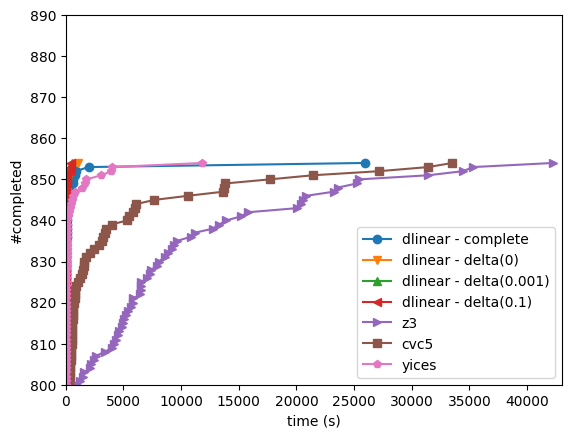
\includegraphics[width=\linewidth]{img/on_file_lp.png}
        \caption{Results over problems completed by all solvers}
        \label{fig:results-lp1}
    \end{subfigure}%
    \hspace{1cm}
    \begin{subfigure}{.45\textwidth}
        \centering
        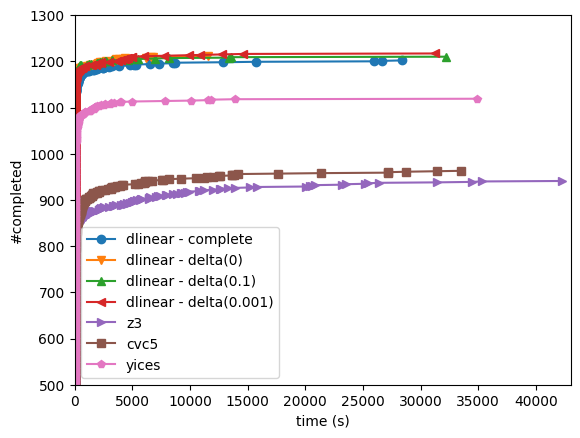
\includegraphics[width=\linewidth]{img/total_lp.png}
        \caption{Results over all problems}
        \label{fig:results-lp2}
    \end{subfigure}
\end{figure}

\begin{table}
    \vspace{-1cm}
    \scriptsize
    \begin{tabular*}{\textwidth}{@{\extracolsep{\fill}}lrrrrrrrrr}
        \toprule
        &        & \multicolumn{2}{c}{$\text{dlinear}_{\text{c}}$} & \multicolumn{2}{c}{z3} & \multicolumn{2}{c}{cvc5} & \multicolumn{2}{c}{yices} \\
        \cmidrule(l){3-4}\cmidrule(l){5-6}\cmidrule(l){7-8}\cmidrule(l){9-10}
        Test set & \numinstcol & \hspace*{1.5em}\numsolved & \avgtime & \hspace*{1.5em}\numsolved & \avgtime & \hspace*{1.5em}\numsolved & \avgtime & \hspace*{1.5em}\numsolved & \avgtime \\
        \midrule
        all                           & 1237 & 1194 & 1.21 & 934 & 1.35 & 955 & 3.79 & 1111   & 0.31  \\
        common                        & 847  & 847  & 0.62 & 847 & 0.94 & 847 & 2.35 & 847    & 0.10  \\
        \bottomrule
    \end{tabular*}
    \medskip
    \caption{Comparison between all complete solvers over the \gls{smt} problems. \avgtime represents the geometric mean of the time to solve each instance, in seconds.}
    \label{tab:results-lp-complete}
    \vspace{-1cm}
\end{table}

\begin{table}
    \scriptsize
    \begin{tabular*}{\textwidth}{@{\extracolsep{\fill}}lrrrrrrrrr}
        \toprule
        &        & \multicolumn{2}{c}{$\text{dlinear}_{\text{c}}$} & \multicolumn{2}{c}{$\text{dlinear}_{\delta = 0}$} & \multicolumn{2}{c}{$\text{dlinear}_{\delta = 0.001}$} & \multicolumn{2}{c}{$\text{dlinear}_{\delta = 0.1}$} \\
        \cmidrule(l){3-4}\cmidrule(l){5-6}\cmidrule(l){7-8}\cmidrule(l){9-10}
        Test set & \numinstcol & \hspace*{1.5em}\numsolved & \avgtime & \hspace*{1.5em}\numsolved & \avgtime & \hspace*{1.5em}\numsolved & \avgtime & \hspace*{1.5em}\numsolved & \avgtime \\
        \midrule
        all                           & 1237 & 1194 & 1.21 & 1203 & 0.75 & 1209 & 0.72 & 1202   & 0.68  \\
        common                        & 847  & 847  & 0.62 & 847 & 0.38 & 847 & 0.36 & 847    & 0.36  \\
        \bottomrule
    \end{tabular*}
    \medskip
    \caption{Comparison between \dlinear over the \gls{smt} problems with different $\delta$. \avgtime represents the geometric mean of the time to solve each instance, in seconds.}
    \label{tab:results-lp-delta}
    \vspace{-1cm}
\end{table}

\subsection*{SMT Result}

A similar setup was used to run the benchmarks over standard \gls{smt} \gls{qf-lra} problems from the SMT-LIB benchmarking suite~\footnote{\url{https://smt-lib.org/benchmarks.shtml}}.
The results are shown in~\autoref{fig:results-smt1} and \autoref{fig:results-smt2} and summarised in~\autoref{tab:results-smt-complete} and \autoref{tab:results-smt-delta}.
Needless to say, in complete mode the outputs are consistent among all four solvers.
While still not as fast as the more established tools, \dlinear shows some notable performance gains when producing a $\delta$-complete output, managing to outperform Z3.

\begin{figure}[H]
    \centering
    \begin{subfigure}{.46\textwidth}
        \centering
        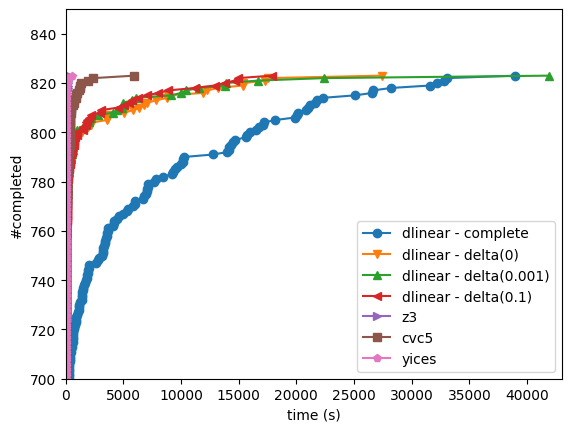
\includegraphics[width=\linewidth]{img/on_file_smt.png}
        \caption{Results over problems completed by all solvers}
        \label{fig:results-smt1}
    \end{subfigure}%
    \hspace{1cm}
    \begin{subfigure}{.45\textwidth}
        \centering
        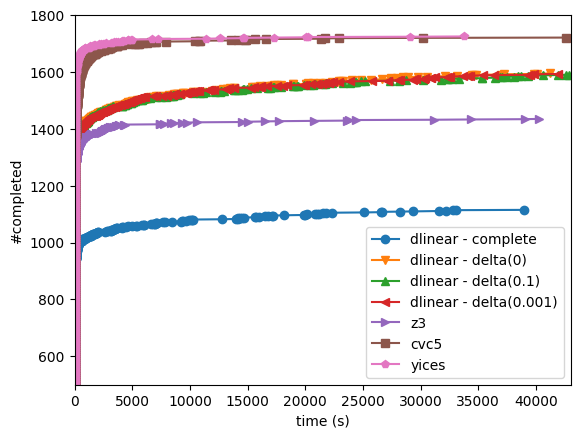
\includegraphics[width=\linewidth]{img/total_smt.png}
        \caption{Results over all problems}
        \label{fig:results-smt2}
    \end{subfigure}
\end{figure}

\begin{table}
    \vspace{-1cm}
    \scriptsize
    \begin{tabular*}{\textwidth}{@{\extracolsep{\fill}}lrrrrrrrrr}
        \toprule
        &        & \multicolumn{2}{c}{$\text{dlinear}_{\text{c}}$} & \multicolumn{2}{c}{z3} & \multicolumn{2}{c}{cvc5} & \multicolumn{2}{c}{yices} \\
        \cmidrule(l){3-4}\cmidrule(l){5-6}\cmidrule(l){7-8}\cmidrule(l){9-10}
        Test set & \numinstcol & \hspace*{1.5em}\numsolved & \avgtime & \hspace*{1.5em}\numsolved & \avgtime & \hspace*{1.5em}\numsolved & \avgtime & \hspace*{1.5em}\numsolved & \avgtime \\
        \midrule
        all                           & 1754 & 1115 & 0.26 & 1435 & 0.85 & 1721 & 1.22 & 1725 & 0.08  \\
        common                        & 823  & 823  & 0.74 & 823  & 0.07 & 823  & 0.22 & 823  & 0.01  \\
        \bottomrule
    \end{tabular*}
    \medskip
    \caption{Comparison between all complete solvers over the \gls{lp} problems. \avgtime represents the geometric mean of the time to solve each instance, in seconds.}
    \label{tab:results-smt-complete}
    \vspace{-1cm}
\end{table}
\begin{table}
    \scriptsize
    \begin{tabular*}{\textwidth}{@{\extracolsep{\fill}}lrrrrrrrrr}
        \toprule
        &        & \multicolumn{2}{c}{$\text{dlinear}_{\text{c}}$} & \multicolumn{2}{c}{$\text{dlinear}_{\delta = 0}$} & \multicolumn{2}{c}{$\text{dlinear}_{\delta = 0.001}$} & \multicolumn{2}{c}{$\text{dlinear}_{\delta = 0.1}$} \\
        \cmidrule(l){3-4}\cmidrule(l){5-6}\cmidrule(l){7-8}\cmidrule(l){9-10}
        Test set & \numinstcol & \hspace*{1.5em}\numsolved & \avgtime & \hspace*{1.5em}\numsolved & \avgtime & \hspace*{1.5em}\numsolved & \avgtime & \hspace*{1.5em}\numsolved & \avgtime \\
        \midrule
        all                          & 1754 & 1115 & 0.26 & 1595 & 0.52 & 1593 & 0.64 & 1591 & 0.68 \\
        common                       & 823  & 823  & 0.74 & 823  & 0.15 & 823  & 0.18 & 823  & 0.2  \\
        \bottomrule
    \end{tabular*}
    \medskip
    \caption{Comparison between \dlinear over the \gls{lp} problems with different $\delta$. \avgtime represents the geometric mean of the time to solve each instance, in seconds.}
    \label{tab:results-smt-delta}
    \vspace{-1cm}
\end{table}

\section{Conclusion}

\dlinear novelty comes from the adoption of exact but not purely rational linear programming solvers adapted for the \gls{smt} context, improving the average performance when dealing with instances where determining the feasibility of the linear constraints represents the main performance bottleneck.
It is able to provide complete verification for problems within the \gls{qf-lra} logic and extends its capabilities to verify neural networks with piecewise activation functions.
The $\delta$-complete approach can further speed up the verification process at the cost of relaxing the constraints by a positive user-defined value.
Future developments will focus on improving the performance of the software by introducing a specialized and efficient symbolic representation of the constraints and improving the heuristics used during the preprocessing phase and the exploration of the search space, especially for neural network verification.

The latest version of the tool is available at \url{https://github.com/TendTo/dlinear}, along with the source code and the technical documentation.
We also provide a corresponding Python API in the form of the \textit{pydlinear} package, to facilitate its installation and use as a library, as well as a Docker image containing the prebuilt binary, making the tool effectively available on any platform supporting containerization.

\begin{credits}
    \subsubsection{\ackname} This study was funded by EPSRC
\end{credits}

% ---- Bibliography ----
\bibliographystyle{splncs04}
\bibliography{resources}

% ---- Appendices ----
% \newpage
% \begin{subappendices}
%     \renewcommand{\thesection}{\Alph{section}}%
%     \section{Proof of~\autoref{thm:lp-relaxed}}
%     \begin{proof}
%         Without loss of generality, assume that both linear programming problems are in standard form.
%         Let $K$ be the set of indexes of strict inequality constraints.
%         \\
%         \framedtext{\eqref{eq:lp-original} feasible $\implies$~\eqref{eq:lp-relaxed} feasible $\land$~\eqref{eq:lp-relaxed} objective value $> 0$} \\

%         If the original problem is feasible, then there exists a solution, a set of values to be assigned to the decision variables $x_1, x_2, \ldots, x_n$, that satisfies all the constraints.
%         For each strict inequality constraint to be satisfied, it means that there exists a value $\delta_k > 0, \quad k \in K$ such that
%         \begin{align*}
%             \sum_{i=1}^{n} a_{ki}x_{i} + \delta_k = b_k, \quad \forall k \in K
%         \end{align*}
%         Let $\bar{t} = \min(\delta_k), \quad k \in K$.
%         Then we know that
%         \begin{align*}
%             \sum_{i=1}^{n} a_{ki}x_{i} + \bar{t} \le b_k, \quad \forall k \in K \\
%             \bar{t} > 0
%         \end{align*}
%         which is the formulation of the strict constraints used in the relaxed problem.
%         All other constraints have been left unchanged, therefore the solution to the original problem can be used to satisfy the constraints of the relaxed problem by setting $t = \bar{t}$, which is greater than $0$.
%         Hence, the objective value of the relaxed problem is $> 0$.
%         \\
%         \framedtext{\eqref{eq:lp-relaxed} feasible $\land$~\eqref{eq:lp-relaxed} objective value $> 0$ $\implies$ \eqref{eq:lp-original} feasible} \\

%         The solution to the relaxed problem already satisfies all the non-strict constraints of the original problem.
%         The objective value is greater than $0$; therefore, $t > 0$.
%         Since all relaxed constraints in the form
%         \begin{align*}
%             \sum_{i=1}^{n} a_{ki}x_{i} + t \le b_k, \quad \forall k \in K \\
%             t > 0
%         \end{align*}
%         are satisfied the original strict inequality constraints
%         \begin{align*}
%             \sum_{i=1}^{n} a_{ki}x_{i} < b_k, \quad \forall k \in K
%         \end{align*}
%         are also satisfied.
%         Hence, the original problem is feasible.
%     \end{proof}

%     % ---- Extended benchmark results (LP) ----
%     \newpage
%     \section{Extended benchmark results}
%     \setlength\LTleft{0pt}
%     \setlength\LTright{0pt}
%     \begin{longtable}{@{\extracolsep{\fill}}lrlrlrlrrrrr@{}}
%         \caption{
%             Extended benchmark results over the \gls{lp} problems in alphabetical order.
%             \textit{res} is the result solvers obtained on that input file. Complete solutions are prioritized over $\delta$-complete ones.
%             The \deltaresult column indicates whether a $\delta$-complete model was found.
%             Finally, \smttime represents the amount of time the solver took to produce an output, in seconds.
%         }                                                                                                                                                                                                                                                                                                     \\
%         \toprule
%               &              & \multicolumn{2}{c}{$\text{dlinear}_{\delta = 0}$} & \multicolumn{2}{c}{$\text{dlinear}_{\delta = 0.001}$} & \multicolumn{2}{c}{$\text{dlinear}_{\delta = 0.1}$} & $\text{dlinear}_{c}$ & z3                & cvc5        & yices                                               \\
%         \cmidrule(l){3-4}\cmidrule(l){5-6}\cmidrule(l){7-8}\cmidrule(l){9-9}\cmidrule(l){10-10}\cmidrule(l){11-11}\cmidrule(l){12-12}
%         File  & \textit{res} & \quad\deltaresult                                 & \smttime                                              & \quad\deltaresult                                   & \smttime             & \quad\deltaresult & \smttime    & \smttime   & \smttime & \smttime & \smttime         \\
%         \midrule
%         \endfirsthead
%         \toprule
%               &              & \multicolumn{2}{c}{$\text{dlinear}_{\delta = 0}$} & \multicolumn{2}{c}{$\text{dlinear}_{\delta = 0.001}$} & \multicolumn{2}{c}{$\text{dlinear}_{\delta = 0.1}$} & $\text{dlinear}_{c}$ & z3                & cvc5        & yices                                               \\
%         \cmidrule(l){3-4}\cmidrule(l){5-6}\cmidrule(l){7-8}\cmidrule(l){9-9}\cmidrule(l){10-10}\cmidrule(l){11-11}\cmidrule(l){12-12}
%         File  & \textit{res} & \quad\deltaresult                                 & \smttime                                              & \quad\deltaresult                                   & \smttime             & \quad\deltaresult & \smttime    & \smttime   & \smttime & \smttime & \smttime         \\
%         \midrule
%         \endhead
%         \csvreader[head to column names]{data/lp.csv}{}
%         {                                                                                                                                                                                                                                                                                                     \\
%         \file & \result      & \quad \resultDO                                   & \smtTimeDO                                            & \quad \resultDOOOI                                  & \smtTimeDOOOI        & \quad \resultDOI  & \smtTimeDOI & \smtTimeDc & \timeZ   & \timeC   & \timeY         }
%     \end{longtable}
%     \newpage
%     \setlength\LTleft{-2cm}
%     \setlength\LTright{0pt}
%     \begin{landscape}
%         \begin{longtable}{@{\extracolsep{\fill}}lrlrlrlrrrrr@{}}
%             \caption{
%                 Extended benchmark results over the \gls{smt} problems in alphabetical order.
%                 \textit{res} is the result solvers obtained on that input file. Complete solutions are prioritized over $\delta$-complete ones.
%                 The \deltaresult column indicates whether a $\delta$-complete model was found.
%                 Finally, \smttime represents the amount of time the solver took to produce an output, in seconds.
%             }                                                                                                                                                                                                                                                                                                     \\
%             \toprule
%                   &              & \multicolumn{2}{c}{$\text{dlinear}_{\delta = 0}$} & \multicolumn{2}{c}{$\text{dlinear}_{\delta = 0.001}$} & \multicolumn{2}{c}{$\text{dlinear}_{\delta = 0.1}$} & $\text{dlinear}_{c}$ & z3                & cvc5        & yices                                               \\
%             \cmidrule(l){3-4}\cmidrule(l){5-6}\cmidrule(l){7-8}\cmidrule(l){9-9}\cmidrule(l){10-10}\cmidrule(l){11-11}\cmidrule(l){12-12}
%             File  & \textit{res} & \quad\deltaresult                                 & \smttime                                              & \quad\deltaresult                                   & \smttime             & \quad\deltaresult & \smttime    & \smttime   & \smttime & \smttime & \smttime         \\
%             \midrule
%             \endfirsthead
%             \toprule
%                   &              & \multicolumn{2}{c}{$\text{dlinear}_{\delta = 0}$} & \multicolumn{2}{c}{$\text{dlinear}_{\delta = 0.001}$} & \multicolumn{2}{c}{$\text{dlinear}_{\delta = 0.1}$} & $\text{dlinear}_{c}$ & z3                & cvc5        & yices                                               \\
%             \cmidrule(l){3-4}\cmidrule(l){5-6}\cmidrule(l){7-8}\cmidrule(l){9-9}\cmidrule(l){10-10}\cmidrule(l){11-11}\cmidrule(l){12-12}
%             File  & \textit{res} & \quad\deltaresult                                 & \smttime                                              & \quad\deltaresult                                   & \smttime             & \quad\deltaresult & \smttime    & \smttime   & \smttime & \smttime & \smttime         \\
%             \midrule
%             \endhead
%             \csvreader[head to column names]{data/smt.csv}{}
%             {                                                                                                                                                                                                                                                                                                     \\
%             \file & \result      & \quad \resultDO                                   & \smtTimeDO                                            & \quad \resultDOOOI                                  & \smtTimeDOOOI        & \quad \resultDOI  & \smtTimeDOI & \smtTimeDc & \timeZ   & \timeC   & \timeY         }
%         \end{longtable}
%     \end{landscape}

% \end{subappendices}

\end{document}
